\chapter[Experimentos e Análise dos Resultados]{Experimentos e Análise dos Resultados}

Nesta seção, são apresentados os experimentos conduzidos para avaliar o desempenho dos modelos de classificação propostos para a detecção automática de dor com base na \textit{Mouse Grimace Scale}, bem como para investigar o impacto de diferentes escolhas de modelagem na capacidade de generalização dos classificadores.

Com o objetivo de garantir a comparabilidade entre os resultados, os modelos avaliados foram padronizados quanto aos parâmetros de entrada e à forma de distribuição dos dados. Essa padronização minimiza a influência de variações na amostragem e permite que as diferenças de desempenho observadas sejam atribuídas, predominantemente, às características estruturais e ao comportamento de aprendizado das arquiteturas analisadas.

O procedimento experimental foi estruturado em três etapas principais, organizadas de forma progressiva. Na etapa inicial, buscou-se verificar a capacidade dos modelos de aprender padrões a partir dos dados. Essa avaliação foi realizada por meio do monitoramento da redução da função de perda ao longo do treinamento, indicando o correto funcionamento do pipeline de processamento e dos mecanismos de otimização. Essa fase foi conduzida em condições controladas, utilizando um subconjunto reduzido de dados, com foco na validação do pipeline, e não no desempenho absoluto dos modelos.

Na segunda etapa, foi realizada a exploração dos hiperparâmetros, com o objetivo de identificar configurações mais adequadas para cada arquitetura. Os experimentos foram conduzidos em escala intermediária, utilizando o conjunto de dados completo e ampliando gradualmente as épocas de treinamento, bem como a complexidade em relação à fase anterior. Adicionalmente, foram analisadas as curvas de aprendizado, permitindo avaliar a estabilidade do processo de treinamento e identificar possíveis indícios de \textit{overfitting} (sobreajuste) ou \textit{underfitting} (subajuste).

Por fim, na terceira etapa, os modelos foram treinados com foco na maximização da capacidade de generalização. O número de épocas foi definido com base na estabilização das métricas de validação, bem como na identificação de platôs de desempenho ao longo do treinamento. As seções subsequentes apresentam uma descrição detalhada dos cenários experimentais considerados, incluindo as configurações adotadas e uma análise crítica dos resultados obtidos.

\section{Experimento 1 - Implementação e Validação dos Modelos Selecionados}

O primeiro experimento teve como finalidade implementar e validar a operação dos modelos selecionados neste estudo, assegurando que sua construção esteja consistente com as especificações descritas na literatura original. Para isso, foram consideradas como referência as propostas de \cite{he2016} para os modelos da família \textit{ResNet}, \cite{Howard2017} para a arquitetura \textit{MobileNet}, \cite{Huang2017} para a \textit{DenseNet} e \cite{dosovitskiy2020vit} para a arquitetura \textit{Vision Transformer} (\acs{VIT}).

Este experimento atua como uma etapa de validação preliminar, viabilizando a identificação precoce de possíveis inconsistências, tais como falhas no carregamento e processamento dos dados, instabilidades numéricas durante o treinamento (como explosão ou desaparecimento do gradiente), erros no cálculo e registro das métricas, bem como comportamentos anômalos das arquiteturas. Nesse contexto, o objetivo não foi avaliar o desempenho absoluto dos modelos, mas verificar sua capacidade de aprender a partir dos dados e apresentar comportamento consistente durante o processo de otimização.

Para isso, o treinamento foi executado utilizando um subconjunto reduzido da base de dados e um número limitado de épocas. A validação foi considerada satisfatória quando observada uma tendência de convergência, evidenciada pela redução progressiva da função de perda e pelo aumento da acurácia ao longo do treinamento. Dessa forma, foi possível obter evidências de que os componentes responsáveis pelo carregamento dos dados, propagação direta, retropropagação dos gradientes e atualização dos parâmetros estavam operando corretamente.

\subsection{Modelos da Arquitetura \textit{ResNet}}

O trabalho de \cite{he2016} apresenta a configuração estrutural de diferentes variantes da arquitetura \textit{ResNet}, que se distinguem principalmente pela profundidade da rede. No contexto deste estudo, a seleção dos modelos considerou as o tamanho reduzido do conjunto de dados e a baixa complexidade de classificação da tarefa proposta, optando-se por arquiteturas de menor e média profundidade.

Dessa forma, foram selecionadas as variantes \textit{ResNet-18}, \textit{ResNet-34} e \textit{ResNet-50}, por apresentarem um equilíbrio adequado entre capacidade de representação e custo computacional. A organização estrutural desses modelos segue as especificações descritas na literatura original, conforme apresentado na Tabela \ref{tab:resnet_variants_structure}.

\begin{table}[h]
	\centering
	\caption{Comparação estrutural dos diferentes modelos variantes da arquitetura \textit{ResNet}.}
	\label{tab:resnet_variants_structure}
	\renewcommand{\arraystretch}{1.1}
	
	\resizebox{\textwidth}{!}{
	\begin{tabular}{l|c|c|c|c}
		
		\toprule
		\textbf{Camada} & \textbf{ResNet-10} & \textbf{ResNet-18} & \textbf{ResNet-34} & \textbf{ResNet-50} \\
		
		\midrule
		
		Conv1 
		& \multicolumn{4}{c}{$7 \times 7$, 64, stride 2, output: $112 \times 112$} \\
		
		MaxPool 
		& \multicolumn{4}{c}{$3 \times 3$, stride 2, output: $56 \times 56$} \\
		
		\hline
		
		Conv2\_x 
		& $\left[\begin{array}{l} 3\times3, 64 \\ 3\times3, 64 \end{array}\right] \times 1$
		& $\left[\begin{array}{l} 3\times3, 64 \\ 3\times3, 64 \end{array}\right] \times 2$
		& $\left[\begin{array}{l} 3\times3, 64 \\ 3\times3, 64 \end{array}\right] \times 3$
		& $\left[\begin{array}{l} 1\times1, 64 \\ 3\times3, 64 \\ 1\times1, 256 \end{array}\right] \times 3$ \\
		
		\hline
		
		Output size 
		& \multicolumn{4}{c}{$56 \times 56$} \\
		
		\hline
		
		Conv3\_x 
		& $\left[\begin{array}{l} 3\times3, 128 \\ 3\times3, 128 \end{array}\right] \times 1$
		& $\left[\begin{array}{l} 3\times3, 128 \\ 3\times3, 128 \end{array}\right] \times 2$
		& $\left[\begin{array}{l} 3\times3, 128 \\ 3\times3, 128 \end{array}\right] \times 4$
		& $\left[\begin{array}{l} 1\times1, 128 \\ 3\times3, 128 \\ 1\times1, 512 \end{array}\right] \times 4$ \\
		
		\hline
		
		Output size 
		& \multicolumn{4}{c}{$28 \times 28$} \\
		
		\hline
		
		Conv4\_x 
		& $\left[\begin{array}{l} 3\times3, 256 \\ 3\times3, 256 \end{array}\right] \times 1$
		& $\left[\begin{array}{l} 3\times3, 256 \\ 3\times3, 256 \end{array}\right] \times 2$
		& $\left[\begin{array}{l} 3\times3, 256 \\ 3\times3, 256 \end{array}\right] \times 6$
		& $\left[\begin{array}{l} 1\times1, 256 \\ 3\times3, 256 \\ 1\times1, 1024 \end{array}\right] \times 6$ \\
		
		\hline
		
		Output size 
		& \multicolumn{4}{c}{$14 \times 14$} \\
		
		\hline
		
		Conv5\_x 
		& $\left[\begin{array}{l} 3\times3, 512 \\ 3\times3, 512 \end{array}\right] \times 1$
		& $\left[\begin{array}{l} 3\times3, 512 \\ 3\times3, 512 \end{array}\right] \times 2$
		& $\left[\begin{array}{l} 3\times3, 512 \\ 3\times3, 512 \end{array}\right] \times 3$
		& $\left[\begin{array}{l} 1\times1, 512 \\ 3\times3, 512 \\ 1\times1, 2048 \end{array}\right] \times 3$ \\
		
		\hline
		
		Output size 
		& \multicolumn{4}{c}{$7 \times 7$} \\
		
		\hline
		
		AvgPool 
		& \multicolumn{4}{c}{Global average pooling ($1 \times 1$)} \\
		
		FC 
		& \multicolumn{4}{c}{Fully connected layer (3 classes)} \\
		
		\bottomrule
	\end{tabular}
	}
	
\end{table}

O modelo \textit{ResNet-10} corresponde a uma variação ainda mais simplificada da arquitetura proposta por \cite{he2016}, embora não tenha sido originalmente apresentada no artigo, ela permitem avaliar se uma redução adicional da complexidade estrutural pode resultar em treinamento mais estável ou melhor capacidade de generalização em cenários caracterizados por conjuntos de dados limitados, justificando sua adoção para este experimento.
 
Essa variante é composta por dez camadas convolucionais e mantém o mesmo princípio estrutural de aprendizado residual e organização modular baseada em \textit{basic blocks} presente nas demais arquiteturas rasas da família \textit{ResNet} — como as variantes \textit{ResNet-18} e \textit{ResNet-34} — diferenciando-se principalmente no número de blocos e, consequentemente, na profundidade total da rede, conforme ilustrado pela Tabela \ref{tab:resnet_variants_structure}.

Para garantir maior fidelidade ao estudo de \cite{he2016}, o treinamento foi conduzido, sempre que possível, seguindo as configurações de parâmetros descritas no trabalho original, sendo realizadas adaptações apenas nos casos em que tais configurações se mostraram incompatíveis com o cenário experimental definido neste projeto.

No que se refere ao pré-processamento dos dados, buscou-se reproduzir o pipeline adotado pelos autores. Inicialmente, as imagens foram redimensionadas de modo que o menor lado fosse amostrado aleatoriamente no intervalo de [256, 480]. Em seguida, foi aplicada uma operação de \textit{random crop} com tamanho fixo de 224×224 \textit{pixels}, acompanhada de espelhamento horizontal aleatório. Por fim, realizou-se a normalização dos dados de entrada de forma canal a canal, utilizando a média e o desvio padrão calculados a partir do conjunto \textit{ImageNet}.

Adicionalmente, conforme descrito em \cite{he2016}, foi empregada a técnica de \textit{Batch Normalization} (\acs{BN}) após cada camada convolucional e antes da aplicação da função de ativação \textit{\acs{ReLU}}. No trabalho original - implementado no \textit{framework} \textit{Caffe} \cite{jia2014caffe} -, a \acs{BN} é definida como uma camada específica, frequentemente acompanhada por uma camada adicional denominada \textit{Scale}, responsável por aplicar os parâmetros aprendíveis de escala e deslocamento. O processo de normalização pode ser descrito pela seguinte expressão:

\begin{equation}
	x_{norm} = \frac{x - \mu}{\sigma}
\end{equation}

$\mu$ e $\sigma$ correspondem, respectivamente, à média e ao desvio padrão estimados para cada canal. Essa normalização tem como objetivo padronizar a distribuição dos dados de entrada, contribuindo para a estabilidade do treinamento.

No contexto deste trabalho, a implementação foi realizada utilizando o \textit{TensorFlow}, no qual a camada \textit{Batch Normalization} já incorpora internamente os parâmetros de escala e deslocamento, além de gerenciar automaticamente as estatísticas necessárias durante as fases de treinamento e inferência. Essa diferença de implementação não altera o princípio fundamental da técnica, mas simplifica sua utilização prática.

Os autores de \cite{he2016} também destacam a não utilização de \textit{dropout}, uma vez que a \textit{Batch Normalization} já exerce um efeito regularizador significativo. Neste experimento o treinamento foi conduzido por um total de 10 épocas, utilizando a base de dados com imagens dos camundongos, além disso, o \textit{batch size} precisou ser reduzido de 256 para 32 considerando limitações de hardware, tamanho da base utilizada e complexidade do problema. O resultado é descrito na Tabela \ref{tab:resnet_sanity_unified}.

% VALORES OBTIDOS DOS EXPERIMENTOS 14,15 e 16 
\begin{table}[h]
	\centering
	\caption{Valores resultantes para cada modelo variante da arquitetura \textit{ResNet}, durante o teste de validação inicial. Importante ressaltar que o objetivo não foi avaliar o desempenho absoluto dos modelos, mas sim, sua tendência de aprendizado.}
	\begin{tabular}{c|cc|cc|cc}
		
		\toprule
		\multirow{2}{*}{\textbf{Época}} 
		& \multicolumn{2}{c|}{\textbf{ResNet-18}} 
		& \multicolumn{2}{c|}{\textbf{ResNet-34}} 
		& \multicolumn{2}{c}{\textbf{ResNet-50}} \\
		
		& Acurácia & Perda & Acurácia & Perda & Acurácia & Perda \\
		
		\midrule
		
		1  & 0.4420 & 1.4406 & 0.4480 & 1.8220 & 0.4456 & 2.8179 \\
		3  & 0.4481 & 1.4252 & 0.4528 & 1.7870 & 0.4788 & 2.7549 \\
		5  & 0.4511 & 1.4145 & 0.4619 & 1.7630 & 0.5007 & 2.6919 \\
		7  & 0.4760 & 1.3939 & 0.4651 & 1.7384 & 0.5221 & 2.6262 \\
		9  & 0.4982 & 1.3735 & 0.4805 & 1.7143 & 0.5172 & 2.5747 \\
		\bottomrule
	\end{tabular}
	\label{tab:resnet_sanity_unified}
\end{table}

Observa-se nos resultados, um comportamento caracterizado pela redução progressiva da função de perda (\textit{loss}) e pelo aumento gradual da acurácia ao longo das épocas. Esse padrão indica uma capacidade consistente de aprendizado, evidenciando o correto funcionamento do pipeline de treinamento, incluindo as etapas de carregamento e pré-processamento dos dados, bem como os mecanismos de otimização empregados. 

Adicionalmente, não foram observadas instabilidades significativas, como explosão ou desaparecimento do gradiente, nem oscilações anômalas nas métricas monitoradas. Embora os valores absolutos de desempenho ainda sejam modestos — o que é esperado, dado o uso de número limitado de épocas —, a tendência consistente de melhoria nas métricas confirma que as arquiteturas estão operando conforme o esperado.

\subsection{Arquiteturas \textit{MobileNet} e \textit{DenseNet}}

Ambas as arquiteturas convolucionais \textit{MobileNet} e \textit{DenseNet} seguiram o mesmo protocolo de validação adotado para a arquitetura \textit{ResNet}. O objetivo desta etapa do experimento permanece o mesmo: permitir a identificação precoce de possíveis inconsistências, instabilidades numéricas ou comportamentos anômalos dos modelos ao longo das 10 épocas de treinamento.

A configuração dos parâmetros buscou, sempre que possível, manter-se alinhada aos trabalhos originais propostos por \cite{Howard2017} e \cite{Huang2017}. No entanto, foram realizadas adaptações específicas, incluindo a redução da resolução de entrada das imagens, a diminuição do tamanho do \textit{batch} e o ajuste da taxa de aprendizado, com o objetivo de tornar o treinamento mais estável e adequado ao cenário experimental deste projeto. A Tabela \ref{tab:unified_training_config} apresenta, os valores dos parâmetros utilizados no experimento.

Apesar dessas modificações, os elementos estruturais fundamentais das arquiteturas foram preservados. Em particular, destacam-se o uso de convoluções separáveis em profundidade na \textit{MobileNet} e o padrão de conectividade densa na \textit{DenseNet}, caracterizado pela taxa de crescimento ($k$) e pelo fator de compressão ($\theta$). A manutenção desses componentes assegura a compatibilidade conceitual aos modelos propostos na literatura.

\begin{table}[h]
	\centering
	\caption{Configuração estrutural dos modelos MobileNet-V1 e DenseNet.}
	\label{tab:unified_training_config}
	\renewcommand{\arraystretch}{1.3}
	
	\begin{tabular}{l | c | c}
		
		\toprule
		\textbf{Parâmetro} & \textbf{DenseNet} & \textbf{MobileNet}\\
		\midrule
		
		Arquitetura / Estrutura 
		& [6, 8, 12, 8] (Blocos Densos) 
		& MobileNet-V1\\
		
		Input size 
		& $128 \times 128 \times 3$ 
		& $160 \times 160 \times 3$\\
		
		\hline
		\makecell[l]{Divisão para o\\conjunto de validação}
		& \multicolumn{2}{c}{0.20} \\
		
		\hline
		
		Função Perda
		& Sparse Categorical CE 
		& Sparse Categorical CE\\
		
		Otimizador 
		& SGD (Nesterov) 
		& RMSprop\\
		
		\textit{Learning Rate} Inicial 
		& $1 \times 10^{-2}$ 
		& $1 \times 10^{-3}$\\
		
		\hline
		
		\textit{Momentum} 
		& \multicolumn{2}{c}{0.9} \\
		
		\hline
		
		\textit{Batch size }
		& 32 
		& 32\\
		
		\hline
		
		Critério de parada
		& \multicolumn{2}{c}{Estabilização no conjunto de validação}\\
		
		\hline
		
		\textit{Hardware} 
		& \multicolumn{2}{c}{Aceleração por GPU  (RTX-3070)}\\
		
		\hline
		
		Multiplicador de Largura
		& - 
		& $\alpha = 0.75$\\
		
		Taxa de Crescimento
		& $k = 24$
		& -\\
		
		Fator de Compressão
		& $\theta = 0.5$ 
		& -\\
		
		\bottomrule
	\end{tabular}
\end{table}

No caso da \textit{MobileNet}, a redução da resolução de entrada (de 224×224 para 160×160) e a utilização de um multiplicador de largura $\alpha = 0.75$ seguem diretamente os mecanismos propostos no artigo original para controle do custo computacional. Já na \textit{DenseNet}, a escolha de uma arquitetura menos profunda e de um valor reduzido para a taxa de aprendizado contribui para maior estabilidade do treinamento em cenários com menor volume de dados, porém mantendo os benefícios associados ao reaproveitamento de características e ao fluxo eficiente de gradientes.

Neste contexto, as modificações aplicadas não comprometem os princípios fundamentais das arquiteturas, mas refletem uma adaptação necessária para garantir a aplicabilidade dos modelos ao contexto do problema estudado. A tabela \ref{tab:mobile_dense_sanity} descreve os valores obtidos durante o treinamento teste.

% VALORES OBTIDOS DOS EXPERIMENTOS 1 (MOBILENET) E 2 (DENSENET)
\begin{table}[H]
	\centering
	\caption{Valores resultantes do teste de validação, conduzido para os modelos \textit{DenseNet} e \textit{MobileNet-V1}.}
	
	\begin{tabular}{c|cc|cc}
		
		\toprule
		\multirow{2}{*}{\textbf{Época}} 
		
		& \multicolumn{2}{c|}{\textbf{MobileNet-V1}} 
		& \multicolumn{2}{c}{\textbf{DenseNet}} \\
		
		& Acurácia & Perda & Acurácia & Perda\\
		\midrule
		1  & 0.6366 & 1.0169 & 0.6461 & 0.7818 \\
		3  & 0.6858 & 1.8312 & 0.7182 & 0.6362 \\
		5  & 0.7151 & 0.7710 & 0.7609 & 0.5464 \\
		7  & 0.7501 & 0.7077 & 0.7905 & 0.4825 \\
		9  & 0.7547 & 0.6821 & 0.8108 & 0.4458 \\
		\bottomrule
	\end{tabular}
	\label{tab:mobile_dense_sanity}
\end{table}

Os resultados apresentam um comportamento característico de um treinamento saudável, justificado pela redução progressiva da função de perda (loss) e pelo aumento gradual da acurácia ao longo das
épocas, o qual indica que os modelos foram capazes de aprender padrões a partir dos dados. Adicionalmente, não foram observadas instabilidades como explosão ou desaparecimento do gradiente, nem oscilações anômalas nas métricas monitoradas.

\subsection{Arquitetura Vision Transformer}

Diferentes variantes da arquitetura \textit{Vision Transformer} foram propostas no trabalho original de \cite{dosovitskiy2020vit}, variando principalmente em profundidade, dimensão dos \textit{embeddings}, número de cabeças de atenção e tamanho dos \textit{patches} utilizados como entrada. As principais configurações apresentadas correspondem aos modelos \textit{\acs{VIT}-Base}, \textit{\acs{VIT}-Large} e \textit{\acs{VIT}-Huge}, que diferem significativamente em capacidade representacional e custo computacional. Conforme descrito pelos autores, o modelo \textit{\acs{VIT}-Base} possui 12 camadas \textit{Transformer} e aproximadamente 86 milhões de parâmetros, enquanto as variantes \textit{Large} e \textit{Huge} ampliam substancialmente essa complexidade, atingindo cerca de 307 milhões e 632 milhões de parâmetros, respectivamente.

A implementação utilizada neste trabalho foi baseada no repositório oficial disponibilizado pela equipe da \textit{Google Research} \cite{vision_transformer_google}. A partir da implementação original, foram realizadas adaptações com o objetivo de preservar exclusivamente os componentes essenciais da arquitetura \acs{VIT}, removendo dependências externas e elementos auxiliares não diretamente relacionados à estrutura central do modelo. O repositório original também disponibiliza pesos pré-treinados obtidos em bases de larga escala, permitindo a utilização de estratégias de \textit{transfer learning} e refinamento (\textit{fine-tuning}) em novos conjuntos de dados.

Considerando o escopo deste estudo, optou-se pela utilização do modelo \textit{\acs{VIT}-B/16}, que apresenta complexidade computacional substancialmente inferior às demais versões apresentadas e a torna mais adequada ao cenário experimental, caracterizado por um conjunto de dados moderado em tamanho e complexidade. Neste contexto, modelos excessivamente parametrizados poderiam apresentar maior risco de \textit{overfitting}, o que reforça a adequação do modelo escolhido. 

Adicionalmente, o valor '16' presente na nomenclatura do modelo refere-se ao tamanho dos \textit{patches} utilizados durante o processo de tokenização da imagem. O valor deste parâmetro influencia diretamente o número de \textit{tokens} processados pelo \textit{Transformer}, afetando tanto a granularidade espacial das informações quanto o custo computacional associado ao mecanismo de autoatenção. De maneira geral, \textit{patches} menores preservam uma quantidade maior de detalhes locais, permitindo uma representação espacial mais refinada da imagem.

Considerando que a \textit{Mouse Grimace Scale} (\acs{MGS}) baseia-se na identificação de alterações faciais sutis associadas à dor, a utilização de \textit{patches} excessivamente grandes poderia comprometer a preservação de características espaciais relevantes para a discriminação das expressões faciais. Nesse contexto, a configuração \textit{\acs{VIT}-B/16} apresenta o melhor balanço entre capacidade de representação espacial e custo computacional, tornando-se compatível com os objetivos e limitações experimentais deste estudo. A configuração completa do modelo encontra-se descrita na Tabela \ref{tab:vit_training_config}.

\begin{table}[h]
	\centering
	\caption{Configuração experimental do modelo \acs{VIT}. A nomenclatura dos parâmetros foi mantida em inglês para assegurar consistência com a terminologia utilizada no artigo original da arquitetura.}
	\label{tab:vit_training_config}
	
	\begin{tabular}{l | c}
		
		\toprule
		\textbf{Parâmetros} & \textbf{Valores}\\
		\midrule
		
		Patch Size
		& 16\\
		
		Embeddings Dimension
		& 768\\
		
		Transform Layers
		& 12\\
		
		Attention Heads 
		& 12\\
		
		\acs{MLP} Units
		& 3072\\
		
		Image Input Size 
		& $(224 \times 224)$\\
		
		Batch Size
		& 16\\
		
		Warmup Steps
		& 1000\\
		
		Base Learning Rate
		& 1e-4\\
		
		Mode
		& Finetune\\
		
		\bottomrule
	\end{tabular}
\end{table}


Devido à utilização da técnica de \textit{Transfer Learning} com a arquitetura \acs{VIT}, determinados parâmetros estruturais da rede precisaram ser mantidos em conformidade com a configuração originalmente proposta por \cite{dosovitskiy2020vit}. Entre esses parâmetros destacam-se o tamanho dos \textit{patches} (\textit{Patch Size}), a dimensão dos \textit{embeddings}, o número de camadas do Transformer (\textit{Transformer Layers}), a quantidade de cabeças de atenção (\textit{Attention Heads}) e a dimensão das camadas do bloco \acs{MLP} (\textit{\acs{MLP} Units}).

A preservação desses valores foi necessária para garantir a compatibilidade entre a arquitetura implementada neste estudo e os pesos pré-treinados disponibilizados no repositório oficial da \textit{Google Research}. Alterações nesses componentes estruturais inviabilizariam o carregamento correto dos pesos previamente treinados, comprometendo a utilização do processo de refinamento (\textit{fine-tuning}) adotado neste trabalho.

% VALORES OBTIDOS DOS EXPERIMENTOS 1 (MOBILENET) E 2 (DENSENET)
\begin{table}[h]
	\centering
	\caption{Resultados do teste de validação conduzido com o modelo \acs{VIT}/B-16.}
	
	\begin{tabular}{l|c|c}
		
		\toprule
		\textbf{Época} & 
		\makecell{\textbf{Perda}\\ \textbf{(Treino)}} &
		\makecell{\textbf{Perda}\\ \textbf{(Validação)}} \\
		
		\midrule
		
		1  & 0.526026657 & 1.035869556\\
		2  & 0.692723343 & 0.773958858\\
		3  & 0.763598703 & 0.677247008\\
		4  & 0.801603026 & 0.589573754\\
		5  & 0.84068804 & 0.5614211\\
		\bottomrule
	\end{tabular}
	\label{tab:vit_sanity}
\end{table}

Os resultados do experimento de validação com a \acs{VIT} - assim como nos demais modelos testados - apresentam uma redução progressiva da função de perda (loss) e um aumento gradual da acurácia ao longo das épocas, ilustrado pela tabela \ref{tab:vit_sanity}. Adicionalmente, não foram observadas instabilidades nem oscilações anômalas nas métricas monitoradas, o que indica um aprendizado efetivo e evidencia o correto funcionamento do pipeline de treinamento, incluindo as etapas de carregamento e pré-processamento dos dados, bem como os mecanismos de otimização empregados. 

Vale destacar que os valores apresentados na Tabela \ref{tab:vit_sanity} indicam uma convergência relativamente acelerada já nas primeiras épocas de treinamento, especialmente considerando o curto intervalo experimental adotado nesta etapa de validação. Embora esse comportamento possa sugerir indícios iniciais de \textit{overfitting}, o objetivo principal deste experimento consiste exclusivamente na validação do pipeline de execução e na verificação da estabilidade operacional do modelo. Aspectos relacionados à capacidade de generalização serão investigados de maneira mais aprofundada nos experimentos posteriores, conduzidos sob regimes de treinamento mais extensos e configurações experimentais mais robustas.

\section{Experimento 2 - Treinamento Conduzido com os Modelos da Arquitetura \textit{ResNet}}

No estudo original de \cite{he2016}, o treinamento foi conduzido utilizando a base de dados \textit{ImageNet}, composta por aproximadamente 1,28 milhão de imagens distribuídas em 1000 classes distintas. Em contraste, o presente trabalho utiliza uma base significativamente menor, composta por cerca de 13 mil imagens rotuladas em três classes, das quais 25\% foram destinadas ao conjunto de validação. Essa diferença em escala e diversidade de dados impõe desafios adicionais ao processo de treinamento, especialmente no que se refere à capacidade de generalização dos modelos e ao risco de \textit{overfitting}.

Nesse contexto, o experimento foi inicialmente conduzido utilizando o modelo \textit{ResNet-50}, o que se justifica por sua profundidade intermediária dentro da família \textit{ResNet}, permitindo um equilíbrio adequado entre sua capacidade de representação e o cenário experimental apresentado. A utilização dessa variante como ponto de partida serve como base para comparações posteriores com variantes mais rasas e outras arquiteturas consideradas neste estudo.

O treinamento foi conduzido por um total de 500 épocas, as demais configuração dos parâmetros de treinamento adotados neste experimento estão sintetizados na Tabela \ref{tab:unified_training_config}, enquanto os detalhes arquiteturais da \textit{ResNet-50} e demais variantes são apresentados na Tabela \ref{tab:resnet_variants_structure}.

De modo geral, os resultados obtidos com a \textit{ResNet-50} mostram-se promissores; em termos quantitativos, o modelo atingiu acurácia média de aproximadamente 86\% tanto no conjunto de treinamento quanto no de validação, o que sugere um processo de aprendizado equilibrado, sem indícios relevantes de \textit{overfitting}. A função de perda convergiu para valores próximos de 1.45, indicando um processo de otimização estável dentro da configuração adotada. Embora o modelo apresente bom desempenho, há espaço para melhorias tanto na acurácia quanto na redução da função de perda, buscando um equilíbrio mais eficiente entre capacidade de aprendizado e generalização.

Considerando o escopo deste estudo — caracterizado por um conjunto de dados de tamanho moderado e por uma tarefa baseada em indicadores bem definidos —, foram conduzidos experimentos adicionais com variantes mais rasas da \textit{ResNet}. Para garantir a consistência da análise, mantiveram-se as mesmas condições experimentais, incluindo a configuração dos hiperparâmetros, o particionamento dos dados e as épocas de treinamento. Essa análise contribui para compreender como a profundidade influencia a capacidade de representação frente à condições mais limitadas.
 
 
\subsection{Utilização de Variantes Rasas da \textit{ResNet}} 

Três arquiteturas adicionais da família \textit{ResNet} foram avaliadas neste experimento, sendo elas: \textit{ResNet-34}, \textit{ResNet-18} e \textit{ResNet-10}, representando configurações progressivamente mais rasas em termos de profundidade. Essa análise complementa os resultados previamente obtidos com a \textit{ResNet-50}, permitindo investigar de forma mais abrangente o impacto da profundidade da rede no desempenho da tarefa proposta. O objetivo central consiste em avaliar em que medida a redução da complexidade estrutural — e, consequentemente, da capacidade representacional — pode ser vantajosa, especialmente em um cenário caracterizado por um conjunto de dados de tamanho moderado. 

Os valores de acurácia e perda reportados para cada variante correspondem às médias calculadas ao longo das 15 últimas épocas, tanto para os conjuntos de treinamento quanto de validação. Essa estratégia foi adotada com o intuito de mitigar flutuações pontuais e garantir que a avaliação reflita um regime de desempenho mais estável, após a fase inicial de convergência. Os resultados quantitativos dos testes encontram-se resumidos na Tabela \ref{tab:comparacao_resnet}, adicionalmente, os gráficos resultantes são apresentados na Figura \ref{fig:resnetcurves}.

Entre os modelos avaliados, as arquiteturas \textit{ResNet-18} e \textit{ResNet-34} apresentaram os resultados mais promissores, considerando o equilíbrio entre os valores de acurácia e da perda. A \textit{ResNet-10}, por sua vez, apresentou uma redução discreta de suas métricas em relação às demais variantes. Embora essa diferença não seja expressiva em termos absolutos, ela evidencia uma tendência de degradação de desempenho associada à redução excessiva da profundidade da rede.

\begin{table}[h]
	\centering
	\caption{Valores resultantes do treinamento conduzido com modelos variantes mais rasos da arquitetura \textit{ResNet}.}
	\label{tab:comparacao_resnet}

		\begin{tabular}{l|c|c|c|c}
			
			\toprule
			\textbf{Modelo} &
			\makecell{\textbf{Acurácia}\\ \textbf{de Treino}} &
			\makecell{\textbf{Acurácia}\\ \textbf{de Validação}} &
			\makecell{\textbf{Perda}\\ \textbf{(Treino)}} &
			\makecell{\textbf{Perda}\\ \textbf{(Validação)}} \\
			
			\midrule
			ResNet-50 & 0.864 & 0.869 & 1.433 & 1.451 \\
			ResNet-34 & 0.912 & 0.895 & 0.714 & 0.800 \\
			ResNet-18 & 0.895 & 0.883 & 0.530 & 0.586 \\
			ResNet-10 & 0.856 & 0.869 & 0.501 & 0.480 \\
			
			\bottomrule
			
		\end{tabular}
\end{table}

\begin{figure}[h]
	\centering
	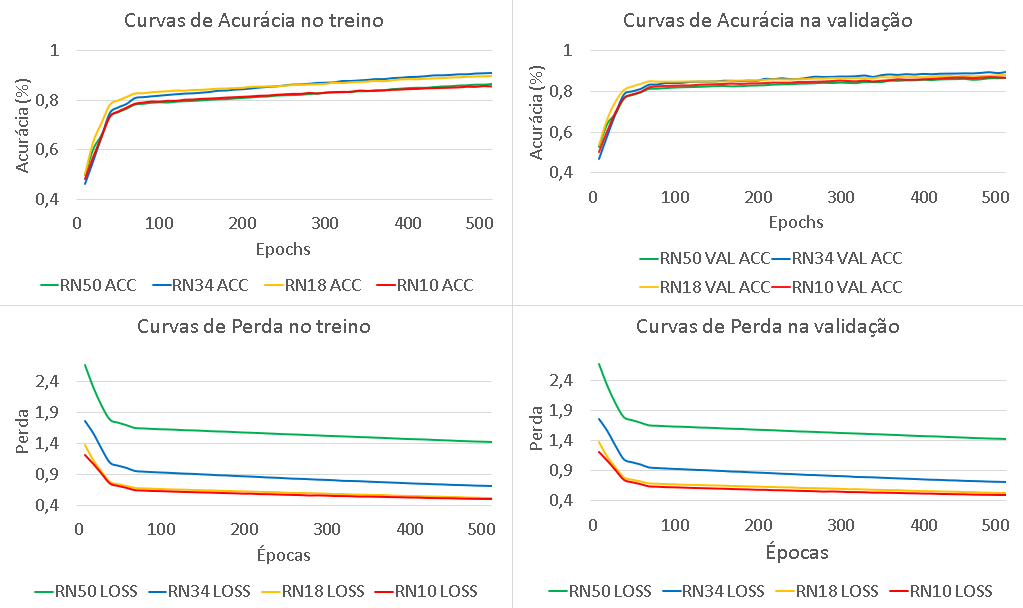
\includegraphics[width=1\linewidth]{figuras/figs_experimentos/resnet_curves}
	\caption{Curvas resultantes do treinamento com os diferentes modelos variantes da arquitetura ResNet. Fonte: o autor.}
	\label{fig:resnetcurves}
\end{figure}

Os resultados obtidos sugerem a existência de um limiar mínimo de complexidade arquitetural necessário para a adequada modelagem do problema. Abaixo desse limiar, a capacidade representacional da rede torna-se insuficiente para capturar relações mais complexas entre as características, limitando o desempenho dos modelos.

Uma vez identificado esse limite estrutural, é importante investigar não apenas a influência da arquitetura, mas também o impacto das configurações de treinamento sobre o desempenho dos modelos, em especial o \textit{batch size} por sua influencia direta sobre a estimativa dos gradientes, o comportamento da convergência. 

\subsection{Avaliação do Impacto do \textit{Batch Size}} 

O tamanho do \textit{batch} desempenha um papel importante na dinâmica de treinamento das redes neurais profundas, influenciando diretamente na capacidade de generalização do modelo. \textit{Batches} menores tendem a introduzir maior variabilidade nas estimativas de gradiente, o que pode atuar como uma forma de regularização implícita, frequentemente resultando em melhor generalização. Por outro lado, \textit{batches} maiores produzem estimativas de gradiente mais estáveis, podendo acelerar a convergência, mas, em alguns casos, levar a uma redução na capacidade de generalização, devido à menor estocasticidade no processo de otimização \cite{keskar2016large}.

Nesse contexto,  foi conduzido um novo conjunto de experimentos focado na análise do impacto do valor de \textit{batch} no desempenho dos modelos mais promissores, definidos no experimento anterior. Para isso, as arquiteturas \textit{ResNet-34} e \textit{ResNet-18} foram novamente treinadas, adotando um aumento no valor do \textit{batch size} de 32 para 64, mantendo-se inalteradas as demais condições experimentais.

Os resultados obtidos com essa nova configuração experimental indicam que valores reduzidos de \textit{batch} se mostraram mais adequados para esse problema, provavelmente devido ao efeito de regularização implícito. Embora o modelo tenha mantido uma dinâmica de treinamento estável, o uso de um \textit{batch} maior não levou a melhorias de desempenho e resultou em uma generalização ligeiramente inferior quando comparado à configuração base, conforme apresentado pela Tabela \ref{tab:comparacao_batchsize_resnet}.

\begin{table}[h]
	\centering
	\caption{Valores resultantes do treinamento conduzido com os modelos \textit{ResNet-18} e \textit{ResNet-34}, considerando um aumento no valor do \textit{Batch Size}.}
	\label{tab:comparacao_batchsize_resnet}
	\setlength{\tabcolsep}{3pt}

		\begin{tabular}{l|c|c|c|c}
			\toprule
			\textbf{Modelo} &
			\makecell{\textbf{Acurácia}\\ \textbf{de Treino}} &
			\makecell{\textbf{Acurácia}\\ \textbf{de Validação}} &
			\makecell{\textbf{Perda}\\ \textbf{(Treino)}} &
			\makecell{\textbf{Perda}\\ \textbf{(Validação)}} \\
			
			\midrule
			
			ResNet-18 (BS = 32)& 0.895 & 0.883 & 0.530 & 0.586 \\
			ResNet-18 (BS = 64) & 0.840 & 0.854 & 0.712 & 0.703 \\
			ResNet-34 (BS = 32)& 0.912 & 0.895 & 0.714 & 0.800 \\
			ResNet-34 (BS = 64) & 0.880 & 0.875 & 0.915 & 0.965 \\
			
			\bottomrule
		\end{tabular}
\end{table}


Um efeito relevante associado à redução do \textit{batch size} é o aumento do número de atualizações de parâmetros realizadas em cada época de treinamento. Como cada atualização passa a utilizar um subconjunto menor de amostras, mais passos de otimização são executados ao longo de cada época, o que pode favorecer uma exploração mais ampla do espaço de parâmetros e facilitar a saída de regiões de mínimo local pouco representativas da função de perda.

Adicionalmente, estudos como o de \cite{masters2018revisiting} indicam que \textit{batches} menores frequentemente apresentam desempenho competitivo ou superior em termos de generalização quando comparados a \textit{batches} maiores, particularmente em cenários nos quais o objetivo principal é maximizar a qualidade preditiva do modelo e não apenas acelerar o processo de treinamento computacional. Com base nesses achados, a configuração com \textit{batch size} igual a 32 foi mantida nos experimentos subsequentes, por apresentar um equilíbrio mais favorável entre estabilidade de convergência e desempenho preditivo. 

% -------------------------------------------------------------------------------
% EXPERIMENTO 6 REFERE-SE AOS SEGUINTES EXPERIMENTOS NA DOCUMENTAÇÃO:
%       •	EXPERIMENTO 14 (RESNET) – TESTE DE 3000 ÉPOCAS COM RESNET18 E BS = 32
% -------------------------------------------------------------------------------

\subsection{Teste Final com a Arquitetura \textit{ResNet}}

Após a identificação das arquiteturas e configurações mais adequadas nos experimentos anteriores, foi conduzido um conjunto final de experimentos com o objetivo de avaliar esses modelos sob um regime de treinamento estendido, totalizando 3000 épocas. O propósito dessa etapa foi investigar se um treinamento prolongado seria capaz de refinar as representações aprendidas, melhorar o desempenho geral dos modelos e, sobretudo, analisar o comportamento de convergência das curvas de aprendizado.

Os resultados, apresentados na Tabela \ref{tab:comparacao_geral} e na Figura \ref{fig:resnetfinal}, indicam que ambas as arquiteturas apresentaram aprendizado consistente e convergência estável ao longo do treinamento. A \textit{ResNet-34} atingiu acurácia máxima de 99,51\% no conjunto de treinamento e 93,74\% no conjunto de validação, enquanto a \textit{ResNet-18} alcançou 99,03\% e 93,42\%, respectivamente. Embora a \textit{ResNet-34} tenha apresentado desempenho ligeiramente superior em termos de acurácia, observa-se que o ganho obtido é marginal.

Em relação à função de perda, a \textit{ResNet-18} apresentou valores mínimos inferiores aos apresentados pela \textit{ResNet-34}, atingindo aproximadamente 0,2424 e 0,5319 para os conjuntos de treinamento e validação, respectivamente. Em contraste, a \textit{ResNet-34} apresentou valores de 0,3768 e 0,7018. Esse resultado sugere que, apesar de sua maior profundidade, a \textit{ResNet-34} não foi capaz de otimizar a função perda de modo mais eficiente nesse cenário específico.

Considerando conjuntamente as métricas de acurácia e perda, bem como a complexidade estrutural dos modelos, a \textit{ResNet-18} destaca-se como a alternativa mais eficiente para a tarefa proposta. Embora a \textit{ResNet-34} apresente ganhos marginais em acurácia, a \textit{ResNet-18} demonstra melhor comportamento de otimização e menor custo computacional, decorrente de sua menor profundidade. Dessa forma, a \textit{ResNet-18} se configura como a escolha mais equilibrada para o problema em estudo, considerando a família de modelos pertencentes à arquitetura \textit{ResNet}.

\begin{figure}[h]
	\centering
	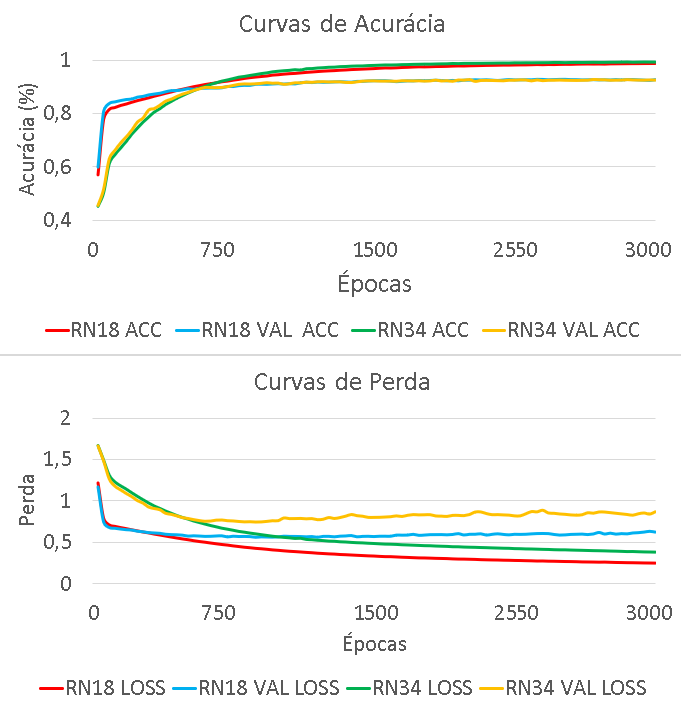
\includegraphics[width=.8\linewidth]{figuras/figs_experimentos/resnet_final}
	\caption{Curvas resultantes do treinamento estendido com as variantes ResNet-18 e ResNet-34. Fonte: o autor.}
	\label{fig:resnetfinal}
\end{figure}


\section{Experimento 3 - Treinamento Conduzido com a Arquitetura \textit{MobileNet}}

Para este experimento, foi conduzido o treinamento da arquitetura \textit{MobileNetV1} com o objetivo de investigar sua eficácia na tarefa de detecção da dor, considerando sua aplicação em cenários com restrições computacionais. Diferentemente de arquiteturas mais profundas e custosas, a \textit{MobileNet} foi projetada para oferecer um bom equilíbrio entre desempenho e eficiência, tornando-se uma alternativa abrangente para implementação em dispositivos com capacidade limitada de processamento.

Embora existam variações mais recentes da arquitetura — como \textit{MobileNetV2} e \textit{MobileNetV3} —, a versão \textit{MobileNetV1} foi selecionada neste estudo por apresentar uma estrutura mais simples e direta, o que facilita a análise isolada do impacto das convoluções separáveis em profundidade. Além disso, por se tratar da formulação original da arquitetura, é possível analisar de forma mais transparente os princípios descritos na literatura \cite{Howard2017}, sem a introdução de mecanismos adicionais, como blocos invertidos ou otimizações específicas de hardware.

Diferentemente das redes convolucionais tradicionais, a \textit{MobileNetV1} utiliza convoluções separáveis em profundidade (\textit{depthwise separable convolutions}), nas quais a operação convolucional padrão é decomposta em duas etapas: uma convolução em profundidade, responsável por aplicar um filtro a cada canal de entrada de forma independente, seguida por uma convolução ponto a ponto, que combina as informações entre os canais. Essa fatoração reduz significativamente o número de parâmetros e o custo computacional do modelo, mantendo sua capacidade de representação.

O modelo adotado segue a arquitetura proposta no trabalho original, no entanto, algumas adaptações foram introduzidas com o objetivo de adequá-lo ao cenário experimental deste estudo, conforme apresentado na Tabela \ref{tab:mobilenet_str}. Dentre as alterações, o multiplicador de largura foi ajustado para $\alpha = 0.75$ a fim de reduzir o número de canais em cada camada e, consequentemente, a complexidade geral do modelo.

Adicionalmente, foi inserida uma camada de \textit{Dropout} com taxa de $0.3$ após a etapa de \textit{global average pooling}, com o intuito de melhorar a capacidade de generalização. Também foi aplicada regularização L2 ($\lambda = 5 \times 10^{-5}$) nas camadas convolucionais e na camada totalmente conectada, buscando reduzir o risco de \textit{overfitting}, especialmente considerando o tamanho reduzido do conjunto de dados utilizado.

Por fim, as imagens de entrada foram redimensionadas para $160 \times 160 \times 3$, buscando um equilíbrio entre preservação da informação espacial e o custo computacional para a \textit{MobileNet}. Demais configurações adotadas para o treinamento encontram-se descritas na Tabela \ref{tab:unified_training_config}. 

\begin{table}[h]
	\centering
	\caption{Resultados médios das últimas 15 épocas no treinamento conduzido com a modelo \textit{MobileNet-V1}}
	\label{tab:results_mobilenet}
	\setlength{\tabcolsep}{3pt}
	
	\begin{tabular}{l|c|c|c|c}
		\toprule
		\textbf{Modelo} &
		\makecell{\textbf{Acurácia}\\ \textbf{de Treino}} &
		\makecell{\textbf{Acurácia}\\ \textbf{de Validação}} &
		\makecell{\textbf{Perda}\\ \textbf{(Treino)}} &
		\makecell{\textbf{Perda}\\ \textbf{(Validação)}} \\
		\midrule
		
		MobileNet - V1 & 0.9920 & 0.8605 & 0.1029 & 1.0241 \\

		\bottomrule
	\end{tabular}
\end{table}

Os resultados apresentados pela Tabela \ref{tab:results_mobilenet}, indicam que o modelo foi capaz de atingir elevada acurácia no conjunto de treinamento ao longo do processo de otimização. A acurácia média nas últimas 15 épocas foi de aproximadamente 99.20\%, com valor correspondente na perda de 0.1029. Entretanto, observa-se uma diferença mais expressiva entre os valores obtidos nos conjuntos de treinamento e validação. A acurácia média de validação atingiu 86.05\%, enquanto a função de perda estabilizou em 1.0241.

Essa discrepância sugere a presença de um leve grau de \textit{overfitting}, no qual o modelo se torna altamente especializado nos dados de treinamento, mas apresenta limitações na capacidade de generalização para dados não vistos. Esse comportamento pode ser atribuído à menor capacidade representacional da arquitetura quando comparada a modelos mais profundos, bem como ao tamanho reduzido do conjunto de dados utilizado.

De modo geral, os resultados indicam que o modelo testado se mostra como uma alternativa viável para cenários nos quais a eficiência computacional é um fator crítico, no entanto, seu desempenho foi inferior ao observado para a arquitetura \textit{ResNet-18} — previamente avaliada neste estudo. Dessa forma, embora a \textit{MobileNetV1} apresente vantagens em termos de custo computacional, sua utilização como modelo principal para a tarefa proposta mostra-se menos vantajosa.

Cabe destacar que foram conduzidos experimentos adicionais com pequenas variações nos hiperparâmetros, a fim de mitigar o \textit{overfitting} observado. No entanto, tais ajustes não resultaram em melhorias significativas. 

\section{Experimento 4 - Treinamento Conduzido com a Arquitetura \textit{DenseNet}}

Neste experimento, foi avaliada uma arquitetura personalizada baseada na \textit{DenseNet}, com o objetivo de investigar o impacto da conectividade densa e do reaproveitamento extensivo de características na tarefa de classificação considerada neste estudo. Diferentemente das redes convolucionais tradicionais, a \textit{DenseNet} estabelece conexões diretas entre todas as camadas dentro de um mesmo bloco denso, permitindo que cada camada receba como entrada os mapas de características de todas as camadas anteriores \cite{Huang2017}.

Esse mecanismo favorece a propagação de informação e gradientes ao longo da rede, além de promover um uso mais eficiente das representações aprendidas. Tais propriedades são relevantes em cenários com conjuntos reduzido de dados e em tarefas que envolvem padrões visuais sutis, como aqueles definidos pela \acs{MGS}, nos quais a preservação de informações em múltiplos níveis de abstração pode contribuir para um melhor desempenho do modelo.

Inicialmente, foram conduzidos testes preliminares utilizando a arquitetura padrão \textit{DenseNet-121}. No entanto, foi proposta uma versão personalizada com o objetivo de reduzir a complexidade computacional do modelo, alinhado com a estratégia adotada no experimento com a \textit{MobileNet}, que buscou avaliar arquiteturas mais eficientes para viabilizar sua implementação em ambientes com restrições computacionais. Uma comparação estrutural das camadas densas entre o modelo base e a configuração customizada proposta é apresentada na Tabela \ref{tab:densenet_comparison}.

\begin{table}[h]
	\centering
	\caption{Comparativo entre o modelo \textit{DenseNet-121} e o modelo customizado mais raso da \textit{DenseNet}.}
	\label{tab:densenet_comparison}
	\renewcommand{\arraystretch}{1.8}
	
	\resizebox{\textwidth}{!}{
		\begin{tabular}{lcc}
			\toprule
			\textbf{Camada} & \textbf{Modelo Customizado} & \textbf{DenseNet-121 (Padrão)} \\
			\midrule
			
			Conv1 
			& $3 \times 3$, 48 filters 
			& $7 \times 7$, 64 filters, stride 2 + MaxPool \\
			
			Dense Block 1 
			& 6 layers, $k=24$ 
			& 6 layers, $k=32$ \\        
			
			Transition 1 
			& $1 \times 1$ conv + AvgPool ($\theta = 0.5$) 
			& $1 \times 1$ conv + AvgPool ($\theta = 0.5$) \\ 
			
			Dense Block 2 
			& 8 layers, $k=24$ 
			& 12 layers, $k=32$ \\        
			
			Transition 2 
			& $1 \times 1$ conv + AvgPool ($\theta = 0.5$) 
			& $1 \times 1$ conv + AvgPool ($\theta = 0.5$) \\
			
			Dense Block 3 
			& 12 layers, $k=24$ 
			& 24 layers, $k=32$ \\
			
			Transition 3 
			& $1 \times 1$ conv + AvgPool ($\theta = 0.5$) 
			& $1 \times 1$ conv + AvgPool ($\theta = 0.5$) \\
			
			Dense Block 4 
			& 8 layers, $k=24$ 
			& 16 layers, $k=32$ \\
			
			\midrule
			
			Batch Normalization + \acs{ReLU} 
			&  \multicolumn{2}{c}{Camada final de normalização seguida por ativação \acs{ReLU} } \\  
			
			AvgPool 
			&  \multicolumn{2}{c}{Camada de extração global das características - Global Average Pooling} \\
			
			Dropout 
			& 0.3 
			& Não utilizado na estrutura padrão \\
			
			Fully Conected 
			& \multicolumn{2}{c}{Camada totalmente conectada} \\
		
			\bottomrule
		\end{tabular}
	}
\end{table}

Os resultados obtidos com ambas as configurações mostraram-se semelhantes, com diferenças marginais tanto em termos de acurácia quanto de perda, conforme descrito na tabela \ref{tab:densenet_variants_results}. Esse comportamento sugere que a capacidade representacional completa da \textit{DenseNet-121} não é estritamente necessária para a tarefa considerada. Dessa forma, optou-se pela utilização da arquitetura personalizada, que apresenta menor custo computacional, mantendo desempenho competitivo.

\begin{table}[h]
	\centering
	\caption{Resultados obtidos pelo treinamento conduzido com ambos os modelos baseados na arquitetura \textit{\textit{DenseNet}} (\textit{DenseNet-121} e \textit{DenseNet} Customizado)}
	\label{tab:densenet_variants_results}
	\setlength{\tabcolsep}{3pt}
	
	\begin{tabular}{l|c|c|c|c}
		\toprule
		\textbf{Modelo} &
		\makecell{\textbf{Acurácia}\\ \textbf{de Treino}} &
		\makecell{\textbf{Acurácia}\\ \textbf{de Validação}} &
		\makecell{\textbf{Perda}\\ \textbf{(Treino)}} &
		\makecell{\textbf{Perda}\\ \textbf{(Validação)}} \\
		\midrule
		
		DenseNet-121 & 0.9985 & 0.9171 & 0.0069 & 0.3707 \\
		DenseNet Customizada & 0.9918 & 0.9182 & 0.0286 & 0.3051 \\

		\bottomrule
	\end{tabular}
\end{table}

Conforme observado no experimento anterior, o processo de treinamento foi interrompido de forma antecipada em função da estabilização das métricas de validação, indicando que o modelo atingiu um regime de convergência no qual variações adicionais nos indicadores de desempenho se tornaram marginais. 

Entretanto, considerando a velocidade elevada de convergência apresentada pela arquitetura \textit{DenseNet}, foi conduzido um experimento adicional utilizando a mesma configuração de treinamento, porém forçando a continuidade do processo até o total de 500 épocas. O objetivo dessa análise consistiu em verificar se a estabilização precoce das métricas correspondia, de fato, a um regime estável de convergência ou se treinamentos mais prolongados poderiam resultar em ganhos adicionais de desempenho. Os resultados correspondentes encontram-se ilustrados na Figura \ref{fig:denseNet500}.

\begin{figure}[h]
	\centering
	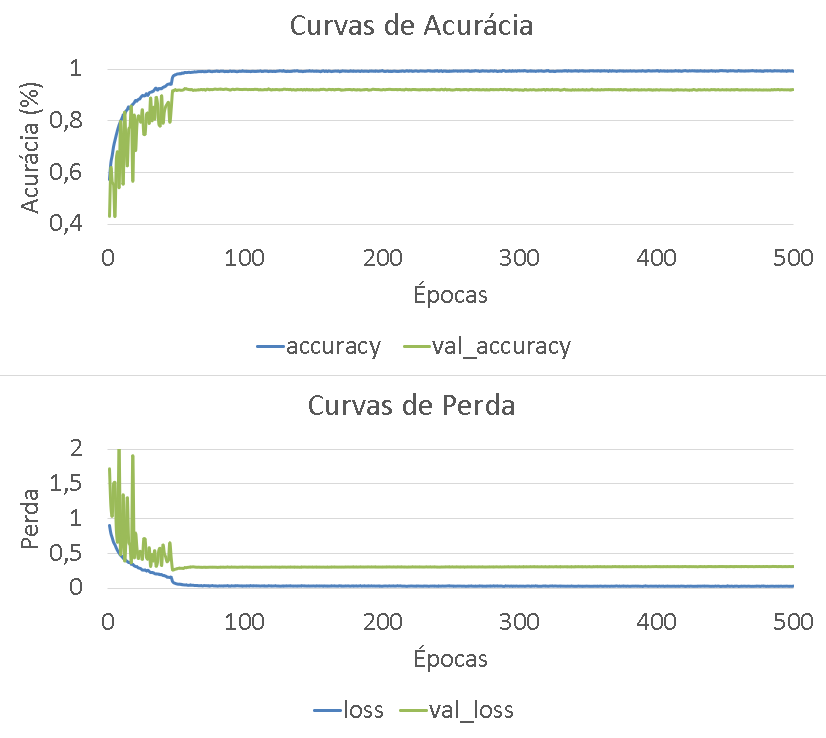
\includegraphics[width=.7\linewidth]{figuras/figs_experimentos/densenet_500eps}
	\caption{Curvas resultantes do treinamento conduzido com a DenseNet por todas as 500 épocas. Fonte: o autor.}
	\label{fig:denseNet500}
\end{figure}

Testes adicionais conduzidos com valores mais elevados de \textit{batch size} resultaram em erros de insuficiência de memória logo nas etapas iniciais do treinamento, inviabilizando a continuidade da execução sob as limitações de hardware disponíveis. As demais configurações de treinamento adotadas encontram-se detalhadas na Tabela \ref{tab:unified_training_config}.

Os resultados obtidos com o modelo customizado, calculados a partir da média das últimas 15 épocas (Tabela \ref{tab:densenet_variants_results}), apresentam um desempenho elevado tanto no conjunto de treinamento quanto no de validação. Diferentemente do que foi observado no experimento conduzido com a \textit{MobileNet}, os valores resultantes nos conjuntos de treino e validação apresentam uma proximidade maior, indicando um processo de aprendizado mais equilibrado e uma capacidade de generalização superior.



Quando comparada às arquiteturas avaliadas anteriormente, a \textit{DenseNet} mantém níveis de acurácia de treinamento semelhantes aos obtidos com a \textit{ResNet}, ao mesmo tempo em que apresenta desempenho superior no conjunto de validação em relação à \textit{MobileNet}, além de um menor desvio entre treinamento e validação. Esses resultados indicam que o mecanismo de reaproveitamento de características contribui fortemente para a captura de padrões visuais sutis associados à dor.

Adicionalmente, considerando os baixos valores de perda observados tanto no treinamento quanto na validação, os resultados sugerem que a arquitetura \textit{DenseNet} modificada apresenta um ajuste mais adequado ao problema proposto. Nesse contexto, o modelo pode ser considerado uma alternativa competitiva e, em alguns aspectos, superior à \textit{ResNet-18}, especialmente no que se refere à capacidade de generalização. 

\section{Experimento 5 - Utilização da Arquitetura \textit{Vision Transformer}}

Neste experimento, foi investigado o comportamento da arquitetura \acs{VIT}, baseada em um paradigma distinto daquele adotado pelas redes convolucionais tradicionais, especialmente no que se refere ao processamento das informações espaciais presentes na imagem. Enquanto as \acsp{CNN} utilizam operações convolucionais para extração hierárquica de padrões locais, os modelos \acs{VIT} tratam a imagem como uma sequência de \textit{patches}, processados por mecanismos de autoatenção (\textit{self-attention}) originalmente propostos para tarefas de processamento de linguagem natural.

A utilização da arquitetura \acs{VIT} é relevante no contexto deste trabalho devido à natureza da \acs{MGS}, cuja avaliação depende da análise conjunta de múltiplas regiões faciais para identificação de expressões sutis associadas à dor. Diferentemente das \acsp{CNN}, os modelos baseados em \textit{Transformers} apresentam menor viés indutivo relacionado à localidade espacial e à invariância translacional, aprendendo essas relações diretamente a partir dos dados durante o treinamento.

Entretanto, essa característica também torna os modelos \acs{VIT} mais dependentes de grandes volumes de dados para treinamento eficiente, especialmente em arquiteturas profundas e altamente parametrizadas. Considerando o tamanho moderado da base de dados utilizada neste estudo, o treinamento foi conduzido utilizando técnicas de \textit{Transfer Learning} e congelamento parcial de camadas (\textit{layer freezing}), empregando pesos pré-treinados na base \textit{ImageNet-21k} para a arquitetura \textit{\acs{VIT}-B/16}, disponibilizados pelo repositório oficial da \textit{Google Research}.

A estratégia de congelamento parcial consistiu em impedir a atualização dos pesos das camadas intermediárias da rede durante o treinamento, permitindo o refinamento apenas das camadas finais responsáveis pela especialização da tarefa. Essa abordagem possibilitou preservar representações visuais gerais previamente aprendidas em bases de larga escala, reduzindo a necessidade de treinamento completo da arquitetura a partir de inicialização aleatória.

Inicialmente, o treinamento foi conduzido durante 500 épocas. Posteriormente, com o objetivo de investigar o comportamento de convergência da arquitetura em treinamentos prolongados, o experimento foi estendido para 800 épocas utilizando a mesma configuração experimental. Os resultados médios obtidos a cada intervalo de 100 épocas são apresentados na Tabela \ref{tab:vit_mean_results_800}.

\begin{table}[h]
	\centering
	\caption{Média dos valores de acurácia e perda obtidos a cada intervalo de 100 épocas durante o treinamento da arquitetura \acs{VIT}.}
	\label{tab:vit_mean_results_800}
	\begin{tabular}{l|c|c|c|c}
		
		\toprule
		\makecell{\textbf{Faixa} \\ \textbf{de épocas}}&
		\makecell{\textbf{Acurácia}\\ \textbf{de treino}} &
		\makecell{\textbf{Acurácia}\\ \textbf{de validação}} &
		\makecell{\textbf{Perda}\\ \textbf{(treino)}} &
		\makecell{\textbf{Perda}\\ \textbf{(validação)}} \\
		\midrule
		
		001-100 & 0.9038 & 0.7519 & 0.4536 & 0.6839 \\
		101-200 & 0.9808 & 0.7982 & 0.3265 & 0.6318 \\
		201-300 & 0.9904 & 0.8212 & 0.3092 & 0.5787 \\
		301-400 & 0.9938 & 0.8255 & 0.3028 & 0.5771 \\
		401-500 & 0.9956 & 0.8239 & 0.2996 & 0.5905 \\
		501-600 & 0.9967 & 0.8204 & 0.2975 & 0.6054 \\
		601-700 & 0.9975 & 0.8262 & 0.2959 & 0.5957 \\
		701-800 & 0.9981 & 0.8354 & 0.2947 & 0.5697 \\
		
		\bottomrule
	\end{tabular}
\end{table}

\begin{comment}
	\begin{table}[h]
		\centering
		\caption{Média dos valores resultantes a cada 100 épocas do treinamento conduzido com a arquitetura \acs{VIT}.}
		\label{tab:vit_mean_results}
		\begin{tabular}{l|c|c|c|c}
			
			\toprule
			\makecell{\textbf{Faixa} \\ \textbf{de épocas}}&
			\makecell{\textbf{Acurácia}\\ \textbf{de Treino}} &
			\makecell{\textbf{Acurácia}\\ \textbf{de Validação}} &
			\makecell{\textbf{Perda}\\ \textbf{(Treino)}} &
			\makecell{\textbf{Perda}\\ \textbf{(Validação)}} \\
			\midrule
			
			001-100 & 0.9046 & 0.7598 & 0.4523 & 0.6577 \\
			101-200  & 0.9808 & 0.79985 & 0.3265 & 0.6296 \\
			201-300 & 0.9909 & 0.8141 & 0.30834 & 0.6065 \\
			301-400 & 0.9946 & 0.8219 & 0.3015 & 0.5908 \\
			401-500 & 0.9966 & 0.8252 & 0.2976 & 0.5916 \\
			
			\bottomrule
		\end{tabular}
	\end{table}
\end{comment}

Os resultados apresentados na Tabela \ref{tab:vit_mean_results_800} correspondem às médias dos valores de acurácia e perda obtidos nos conjuntos de treinamento e validação, calculadas a cada intervalo de 100 épocas. Essa estratégia permite observar de forma mais clara a evolução do desempenho da arquitetura ao longo do treinamento, minimizando oscilações pontuais e evidenciando tendências gerais de convergência.

Observa-se que a arquitetura apresenta rápida convergência nas primeiras 200 épocas, seguida por um regime de estabilização caracterizado por ganhos marginais nas métricas avaliadas. Esse comportamento pode ser parcialmente explicado pela utilização combinada de \textit{Transfer Learning} e congelamento parcial das camadas da rede.

Como a maior parte da arquitetura já havia sido previamente treinada na base \textit{ImageNet-21k}, o modelo iniciou o processo de refinamento com representações visuais previamente estruturadas, reduzindo significativamente a necessidade de aprender padrões básicos a partir de uma inicialização aleatória. Além disso, o congelamento das camadas intermediárias favoreceu a maior estabilidade durante o treinamento e adaptação mais rápida ao domínio específico da tarefa proposta.

Os resultados obtidos indicam que a arquitetura foi capaz de aprender padrões relevantes para a tarefa de classificação, evidenciado pela redução consistente da função de perda e pelo aumento progressivo da acurácia ao longo do treinamento. Entretanto, observa-se um comportamento característico de \textit{overfitting}, uma vez que os elevados valores de acurácia obtidos no conjunto de treinamento não são acompanhados proporcionalmente pelo conjunto de validação, embora este também apresente desempenho satisfatório.

Além disso, o prolongamento do treinamento até 800 épocas produziu ganhos relativamente modestos no desempenho de validação quando comparado às primeiras etapas do treinamento, sugerindo que a arquitetura atinge rapidamente um regime próximo da estabilização para o conjunto de dados utilizado neste estudo. Para melhor visualização do comportamento de convergência da arquitetura, a Figura \ref{fig:vitcurves} apresenta as curvas de acurácia e perda obtidas ao longo do treinamento.


\begin{figure}[h]
	\centering
	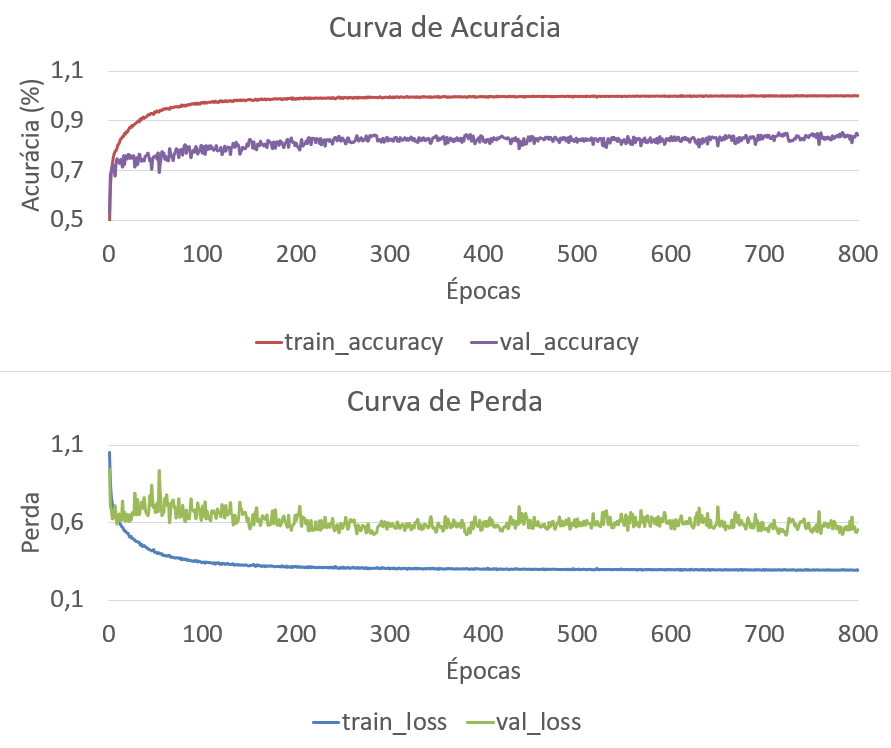
\includegraphics[width=0.8\linewidth]{figuras/figs_experimentos/vit_800eps.png}
	\caption{Curvas de acurácia e perda para o treinamento conduzido com a arquitetura \acs{VIT}. Fonte: o autor.}
	\label{fig:vitcurves}
\end{figure}

\subsection{Treinamento Conduzido com uma Redução no Conjunto de Treino}

O comportamento de \textit{overfitting} observado no experimento anterior sugere que o desempenho da arquitetura \acs{VIT} pode estar diretamente associado à quantidade de dados disponíveis durante o treinamento. Considerando a elevada capacidade representacional dos modelos baseados em \textit{Transformers}, mesmo sob estratégias de \textit{Transfer Learning} e congelamento parcial de camadas, foi conduzido um experimento adicional com redução controlada da base de treinamento, com o objetivo de investigar a sensibilidade da arquitetura à disponibilidade de amostras.

A hipótese considerada neste experimento é que a diminuição da quantidade de dados disponíveis para treinamento reduz a diversidade de padrões visuais apresentados ao modelo, comprometendo sua capacidade de adaptação ao conjunto de validação. Consequentemente, espera-se observar redução dos valores de acurácia e aumento da função de perda durante o processo de avaliação.

Para isso, foi conduzido um novo treinamento utilizando a mesma configuração experimental adotada anteriormente para a arquitetura \acs{VIT}, diferenciando-se apenas pela redução do conjunto de dados destinado ao treinamento. O número de imagens pertencentes a cada classe da base de dados (\textit{Indolor}, \textit{Pouca Dor} e \textit{Muita Dor}) foi reduzido pela metade por meio de remoção aleatória e balanceada das amostras. Essa estratégia permitiu preservar a proporcionalidade entre as classes, evitando a introdução de desequilíbrios que pudessem comprometer a interpretação dos resultados.

Os resultados apresentados na Tabela \ref{tab:vit_reduced_data_mean_results} correspondem às médias dos valores de acurácia e perda obtidos nos conjuntos de treinamento e validação, calculadas a cada intervalo de 100 épocas. Essa abordagem permite observar a evolução do desempenho da arquitetura ao longo do treinamento, minimizando oscilações pontuais nas métricas avaliadas.

\begin{table}[h]
	\centering
	\caption{Média dos valores resultantes a cada 100 épocas do treinamento conduzido com a arquitetura \acs{VIT}, considerando a redução aplicada nas amostras para o conjunto de treino.}
	\label{tab:vit_reduced_data_mean_results}
	\begin{tabular}{l|c|c|c|c}
		
		\toprule
		\makecell{\textbf{Faixa} \\ \textbf{de épocas}}&
		\makecell{\textbf{Acurácia}\\ \textbf{de Treino}} &
		\makecell{\textbf{Acurácia}\\ \textbf{de Validação}} &
		\makecell{\textbf{Perda}\\ \textbf{(Treino)}} &
		\makecell{\textbf{Perda}\\ \textbf{(Validação)}} \\
		\midrule
		
		001-100 & 0.9427 & 0.7458 & 0.3912 & 0.7235 \\
		101-200 & 0.9909 & 0.7591 & 0.3084 & 0.7641 \\
		201-300 & 0.9953 & 0.7639 & 0.3005 & 0.7839 \\
		301-400 & 0.9970 & 0.7671 & 0.2968 & 0.7891 \\
		401-500 & 0.9981 & 0.7761 & 0.2947 & 0.7691 \\
		
		\bottomrule
	\end{tabular}
\end{table}

Os resultados obtidos permanecem consistentes com o comportamento observado no experimento anterior, evidenciando rápida convergência da arquitetura nas primeiras 200 épocas de treinamento, seguida por um regime de estabilização das métricas avaliadas. Entretanto, o comportamento de \textit{overfitting} torna-se significativamente mais pronunciado nesse novo cenário experimental.

Observa-se que, embora a acurácia do conjunto de treinamento permaneça elevada ao longo das épocas, o desempenho obtido no conjunto de validação apresenta redução consistente quando comparado ao experimento conduzido com a base completa. Paralelamente, os valores da função de perda tornam-se progressivamente maiores no conjunto de validação, indicando maior dificuldade da arquitetura em adaptar-se a dados não observados durante o treinamento.

Esses resultados sugerem que, mesmo utilizando estratégias de \textit{Transfer Learning}, as arquiteturas baseadas em \textit{Transformers} permanecem altamente dependentes da disponibilidade de dados para construção de representações robustas. Tal comportamento está alinhado com o observado na literatura, na qual modelos \acs{VIT} frequentemente apresentam maior sensibilidade ao tamanho da base de treinamento quando comparados às arquiteturas convolucionais tradicionais. Para melhor visualização do comportamento de convergência e das diferenças entre os conjuntos de treinamento e validação, a Figura \ref{fig:vitcurves_reduced} apresenta graficamente a evolução das métricas ao longo do treinamento.

\begin{figure}[h]
	\centering
	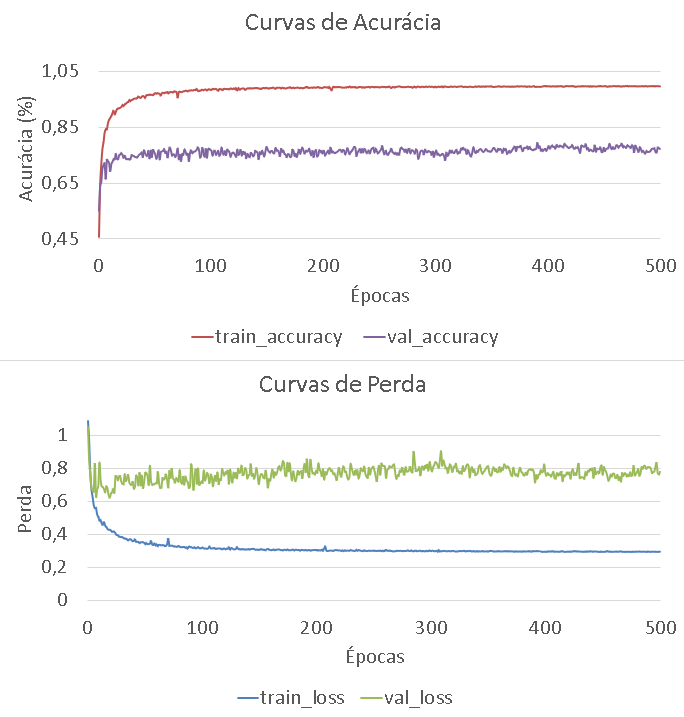
\includegraphics[width=.75\linewidth]{figuras/figs_experimentos/vit_reduced_curves}
	\caption{Curvas de acurácia e perda para o treinamento conduzido com a arquitetura \acs{VIT}, considerando uma redução na base de dados. Fonte: o autor.}
	\label{fig:vitcurves_reduced}
\end{figure}

\subsection{Treinamento Conduzido com uma Alteração na Divisão da Base de Dados}

Além do experimento envolvendo redução controlada da base de treinamento, foi conduzida uma análise adicional com modificação da estratégia de divisão dos subconjuntos de treinamento e validação. O objetivo desse experimento consistiu em investigar o impacto da distribuição das amostras sobre o comportamento das métricas de validação e sobre a estabilidade do processo de avaliação da arquitetura.

Na configuração originalmente adotada com uma divisão de 80/20 por cento, o modelo dispõe de maior quantidade de amostras para aprendizado, favorecendo a construção de representações visuais mais robustas durante o treinamento. Entretanto, em cenários envolvendo bases de dados moderadas — como o presente estudo — conjuntos de validação mais reduzidos podem apresentar maior sensibilidade a flutuações estatísticas, dificultando uma representação mais consistente da variabilidade real dos dados. Dessa forma, optou-se por conduzir um novo experimento utilizando uma divisão de 70/30 entre os conjuntos de treinamento e validação, respectivamente.

Nessa nova configuração, parte das amostras originalmente destinadas ao treinamento passam a compor o conjunto de validação, ampliando a quantidade de exemplos utilizados durante a avaliação do modelo. Embora essa estratégia reduza parcialmente a quantidade de dados disponíveis para aprendizado, ela possibilita uma análise potencialmente mais representativa do comportamento da arquitetura durante a validação.

O treinamento foi conduzido utilizando a mesma configuração experimental adotada anteriormente para a arquitetura \acs{VIT}, diferenciando-se apenas pela nova proporção utilizada na divisão da base de dados. Assim como nos experimentos anteriores, o treinamento foi executado durante 800 épocas, com o objetivo de assegurar estabilização adequada das métricas avaliadas. Os valores médios obtidos a cada intervalo de 100 épocas são apresentados na Tabela \ref{tab:vit_7030_results}.

\begin{table}[h]
	\centering
	\caption{Média dos valores resultantes a cada 100 épocas do treinamento conduzido com a arquitetura \acs{VIT}, considerando a divisão da base de dados 70/30\% para os conjuntos de treino e validação, respectivamente.}
	\label{tab:vit_7030_results}
	\begin{tabular}{l|c|c|c|c}
		
		\toprule
		\makecell{\textbf{Faixa} \\ \textbf{de épocas}}&
		\makecell{\textbf{Acurácia}\\ \textbf{de Treino}} &
		\makecell{\textbf{Acurácia}\\ \textbf{de Validação}} &
		\makecell{\textbf{Perda}\\ \textbf{(Treino)}} &
		\makecell{\textbf{Perda}\\ \textbf{(Validação)}} \\
		\midrule
		
		001-100 & 0.9363 & 0.8070 & 0.4003 & 0.5478 \\
		101-200 & 0.9873 & 0.8447 & 0.3147 & 0.5007 \\
		201-300 & 0.9931 & 0.8553 & 0.3043 & 0.4797 \\
		301-400 & 0.9954 & 0.8617 & 0.2998 & 0.4675 \\
		401-500 & 0.9967 & 0.8645 & 0.2974 & 0.4647 \\
		501-600 & 0.9976 & 0.8637 & 0.2958 & 0.4726 \\
		601-700 & 0.9981 & 0.8685 & 0.2947 & 0.4595 \\
		701-800 & 0.9986 & 0.8715 & 0.2938 & 0.4558 \\
		
		\bottomrule
	\end{tabular}
\end{table}

Os resultados obtidos indicam comportamento semelhante ao observado nos experimentos anteriores, caracterizado por rápida convergência da arquitetura nas primeiras épocas de treinamento, seguida por estabilização gradual das métricas de desempenho. Entretanto, observa-se melhora consistente dos resultados obtidos no conjunto de validação quando comparados à configuração original utilizando divisão 80/20. 

Esse comportamento sugere que o aumento da quantidade de amostras destinadas ao subconjunto de validação contribuiu para uma avaliação mais estável e representativa do desempenho da arquitetura. Ainda assim, deve-se considerar que a redução do conjunto de treinamento também implica menor quantidade de dados disponíveis para aprendizado, configurando um compromisso entre capacidade de treinamento e robustez estatística da validação.

Além disso, embora os resultados indiquem redução relativa do comportamento de \textit{overfitting} quando comparados aos experimentos anteriores, ainda permanece uma diferença significativa entre os desempenhos observados nos conjuntos de treinamento e validação, indicando que a limitação relacionada à disponibilidade de dados continua impactando o comportamento da arquitetura. A Figura \ref{fig:vitcurves_70/30} apresenta as curvas de acurácia e perda obtidas durante o treinamento utilizando a divisão 70/30 da base de dados.

\begin{figure}[h]
	\centering
	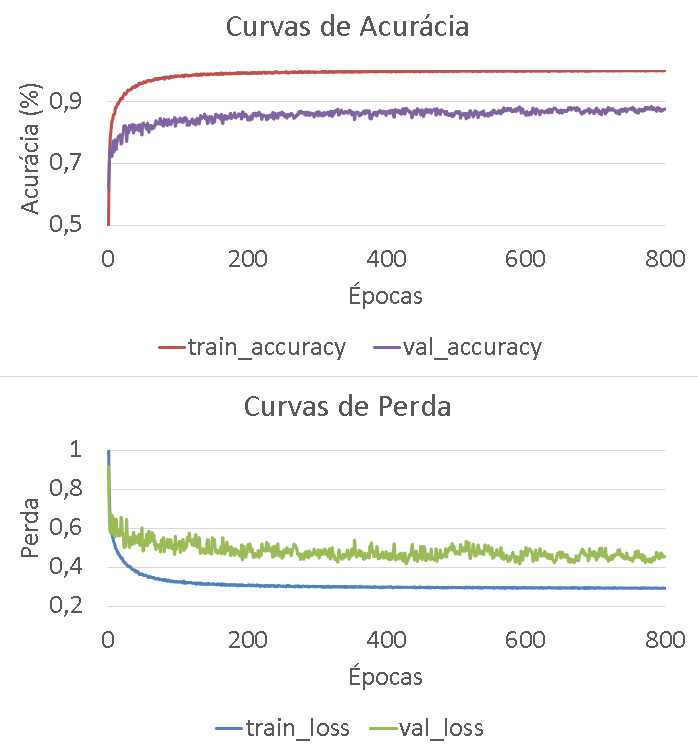
\includegraphics[width=.7\linewidth]{figuras/figs_experimentos/vit_new_data_div}
	\caption{Curvas de acurácia e perda para o treinamento conduzido com a arquitetura \acs{VIT}, considerando a divisão de 70/30 na base de dados. Fonte: o autor.}
	\label{fig:vitcurves_70/30}
\end{figure}

\subsection{Considerações Finais}

Os resultados experimentais obtidos ao longo deste estudo evidenciam aspectos relevantes acerca da aplicabilidade de classificadores neurais para a avaliação automatizada da dor com base na \acs{MGS}. A Tabela \ref{tab:comparacao_geral} apresenta uma visão consolidada dos principais resultados obtidos nos experimentos conduzidos.

Entre os modelos avaliados, as arquiteturas convolucionais fundamentadas no reaproveitamento e na propagação eficiente de características apresentaram desempenho superior. Em especial, os modelos \textit{ResNet}-18 e \textit{DenseNet (Customizado)} obtiveram os melhores resultados gerais, combinando elevados valores de acurácia e expressiva redução na perda. Adicionalmente, observa-se uma forte proximidade nos desempenhos resultantes para os conjuntos de treinamento e validação, o que implica em uma boa capacidade de generalização.

Tais resultados sugerem que mecanismos intensivos de reutilização de características, aliados a um equilíbrio adequado entre profundidade arquitetural e capacidade de representação, constituíram alguns dos principais fatores responsáveis pela eficiência observada na tarefa de classificação proposta. Considerando que as expressões faciais associadas à dor foram caracterizadas por padrões visuais bem definidos, a preservação e reutilização de representações intermediárias ao longo da rede parecem desempenhar um papel importante na melhoria da capacidade de generalização dos modelos.

Além disso, os resultados obtidos com a arquitetura \textit{DenseNet} customizada representam uma contribuição relevante deste trabalho. Embora apresente menor profundidade e complexidade computacional quando comparada ao modelo de referência \textit{DenseNet}-121, a arquitetura proposta foi capaz de manter desempenho competitivo. Dessa forma, a configuração desenvolvida amplia a viabilidade da utilização de estratégias baseadas em conectividade densa, inclusive em cenários caracterizados por restrições computacionais mais severas.

Em contrapartida, embora a arquitetura \textit{MobileNetV1} tenha apresentado comportamento de \textit{overffiting} mais acentuado, com métricas de validação significativamente inferiores às observadas durante o treinamento, seu projeto orientado à eficiência computacional ainda a torna uma alternativa relevante para aplicações em sistemas embarcados e soluções de monitoramento em tempo real. Em cenários nos quais os benefícios proporcionados pela reutilização intensiva de características não se mostrem expressivos, arquiteturas leves como a \textit{MobileNetV1} podem representar um compromisso interessante entre desempenho preditivo e custo computacional.

Outra observação importante refere-se à influência dos parâmetros de configuração do treinamento, especialmente à escolha no tamanho do (\textit{batch size}). Os experimentos conduzidos com as arquiteturas da família \textit{ResNet} indicaram que lotes menores favoreceram o desempenho no conjunto de validação e contribuíram para a redução do \textit{overfitting}, particularmente em bases de dados com tamanho moderado e em tarefas envolvendo padrões faciais sutis.

Esse comportamento pode estar associado ao efeito de regularização implícita decorrente da maior variabilidade presente na estimativa dos gradientes durante o processo de otimização. Tal observação está em conformidade com resultados previamente reportados na literatura de aprendizado profundo, que apontam o uso de lotes menores como um fator potencialmente benéfico para a capacidade de generalização dos modelos.

\begin{table*}[h]
	\centering
	\caption{Resultados agregados dos experimentos conduzidos com as diferentes arquiteturas de redes neurais.}
	\label{tab:comparacao_geral}
	\renewcommand{\arraystretch}{1.3}
	
	\begin{tabular}{l|c|c|c|c|c|c}
		\toprule
		
		\makecell{\textbf{Modelo}}&
		\makecell{\textbf{Épocas}}&
		\makecell{\textbf{Batch}\\ \textbf{Size}}&
		\makecell{\textbf{Acurácia}\\ \textbf{(Treino)}} &
		\makecell{\textbf{Acurácia}\\ \textbf{(Val.)}} &
		\makecell{\textbf{Perda}\\ \textbf{(Treino)}} &
		\makecell{\textbf{Perda}\\ \textbf{(Val.)}} \\
		\midrule

		ResNet-50 & 500 & 32 & 0.864 & 0.869 & 1.433 & 1.451 \\
		ResNet-34 & 3000 & 32 & 0.995 & 0.937 & 0.376 & 0.701 \\
		ResNet-34 & 500 & 64 & 0.880 & 0.875 & 0.915 & 0.965 \\
		ResNet-18 & 3000 & 32 & 0.990 & 0.934 & 0.242 & 0.531 \\
		ResNet-18 & 500 & 64 & 0.840 & 0.854 & 0.712 & 0.703 \\
		ResNet-10 & 500 & 32 & 0.856 & 0.869 & 0.501 & 0.480 \\
		MobileNet-V1 & 500 & 32 & 0.992 & 0.860 & 0.102 & 1.024 \\
		DenseNet-121 & 500 & 16 & 0.998 & 0.917 & 0.006 & 0.370 \\
		DenseNet C. & 500 & 16 & 0.991 & 0.918 & 0.028 & 0.305 \\
		\acs{VIT} & 800 & 16 & 0.998 & 0.835 & 0.294 & 0.569 \\
		\acs{VIT} (70/30) & 800 & 16 & 0.998 & 0.871 & 0.293 & 0.455 \\
		
		\bottomrule
		
	\end{tabular}
\end{table*}

Considerando os experimentos conduzidos com o modelo \acs{VIT}, os resultados evidenciaram a presença consistente de \textit{overfitting}, caracterizada pela diferença relativamente elevada entre os desempenhos observados nos conjuntos de treinamento e validação. Esse comportamento foi observado mesmo com a utilização de \textit{Transfer Learning} a partir de pesos previamente treinados na base \textit{ImageNet-21k}. Adicionalmente, a redução controlada das amostras disponíveis para treinamento reforçou essa observação, resultando em degradação significativa das métricas de validação.

Diferentemente das redes convolucionais tradicionais, que incorporam explicitamente propriedades estruturais importantes para o processamento de imagens — como localidade espacial, compartilhamento de pesos e invariância translacional — os modelos \acs{VIT} não assumem previamente essas relações, como consequência, arquiteturas baseadas em \textit{Transformers} tendem a demandar conjuntos de dados significativamente maiores para alcançar desempenho mais robusto em tarefas de classificação visual.

Esse comportamento sugere que o desempenho da arquitetura está fortemente associado à diversidade e à quantidade de dados disponíveis, característica amplamente reportada na literatura para modelos baseados em \textit{Transformers}. Ainda assim, os resultados obtidos podem ser considerados satisfatórios, especialmente quando se considera o tamanho relativamente limitado da base de dados utilizada e a natureza especializada da tarefa de classificação proposta.

Nesse contexto, o principal fator limitante para a melhoria do desempenho da arquitetura não está necessariamente relacionado à sua capacidade representacional, nem exclusivamente à configuração dos hiperparâmetros empregados, mas sobretudo à disponibilidade de dados para treinamento. Embora estratégias adicionais de otimização possam contribuir para ganhos incrementais de desempenho, a limitação imposta pelo tamanho e pela diversidade do conjunto de dados tende a restringir o potencial máximo da \acs{VIT} no cenário investigado.

Por fim, visando garantir a reprodutibilidade dos resultados obtidos e favorecer a continuidade das pesquisas desenvolvidas nesta área, os códigos-fonte empregados na implementação, treinamento e avaliação dos modelos apresentados nesta dissertação foram disponibilizados no repositório pessoal do autor, na plataforma \textit{GitHub}. O material inclui as implementações das arquiteturas avaliadas, rotinas de pré-processamento dos dados, scripts de treinamento e demais componentes necessários para a reprodução dos experimentos descritos ao longo deste trabalho. 